\section{Evaluation}
\label{sec:evaluation}

We did not compare to other HPC systems because we are not claiming that our
file system metadata protocols are superior. Instead, we use Ceph as a platform
for exploring related work over the same storage system, which facilitates an
apples-to-apples comparison of the strategies themselves.  So we run
experiments on the same cluster and normalize results to control for hardware
differences and to make our results more generally applicable.  Our goal is not
to build a file system optimized for HPC workloads and our prototype is not a
competitor to Lustre. Rather it is a solution for letting the techniques of a
system like Lustre live in the same namespace as techniques optimized for file
creates, like BatchFS. 

\begin{table}
\begin{tabular}{ r | l | l}
  Cluster  & Hardware               & Software \\\hline
  In-House & 15 nodes, 4 2GHz CPUs  & Ubuntu 12.04, 1 MON\\
           & 8GB RAM, SSD           & 1 MDS, 8 OSDs, 8 Clients\\
  CloudLab & 34 nodes, 16 2.4GHz CPUs & Ubuntu 14.04, 1 MON\\
           & 128GB RAM, SSD         & 1 MDS, 3 OSDs, 29 Clients
\end{tabular}
\caption{In-House used for microbenchmarks, CloudLab for Use Cases. MON is
monitor daemon, MDS is metadata server daemon, and OSDs are object storage
daemons.\label{table:clusters}} 
\end{table}

We evaluate our prototype on the two clusters in Table~\ref{table:clusters}.
Microbenchmarks were run on the in-house clusters while client scalability
tests were run on CloudLab. We only scale up to 29 clients because that is the
maximum capacity of a single metadata server. For the in-house cluster, we need
more object storage servers and we have to co-locate clients on the same node
because of resource contention \footnote{The bandwidth to RADOS is only
sufficient with 8 nodes on this older hardware, which uses SSDs and nodes that
are almost 10 years old.  The CloudLab cluster performs just as well with and
without a highly provisioned object storage server cluster.}. All daemons run
as a single process which is the default setting for Ceph. We develop on Ceph's
Jewel release, version 10.2.1, which was released in May 2016.

This paper adheres to The Popper
Convention\footnote{\url{http://falsifiable.us}}~\cite{jimenez_popper_2016}, so
experiments presented here are available in the repository for this
article\footnote{Links have been removed for double-blind submission}.
Experiments can be examined in more detail, or even re-run, by visiting the
\texttt{[source]} link next to each figure. That link points to a Jupyter
notebook that shows the analysis and source code for that graph, which points
to an experiment and its artifacts.

\subsection{Microbenchmarks}
\label{sec:microbenchmarks}
\begin{figure}[tb]
\centering
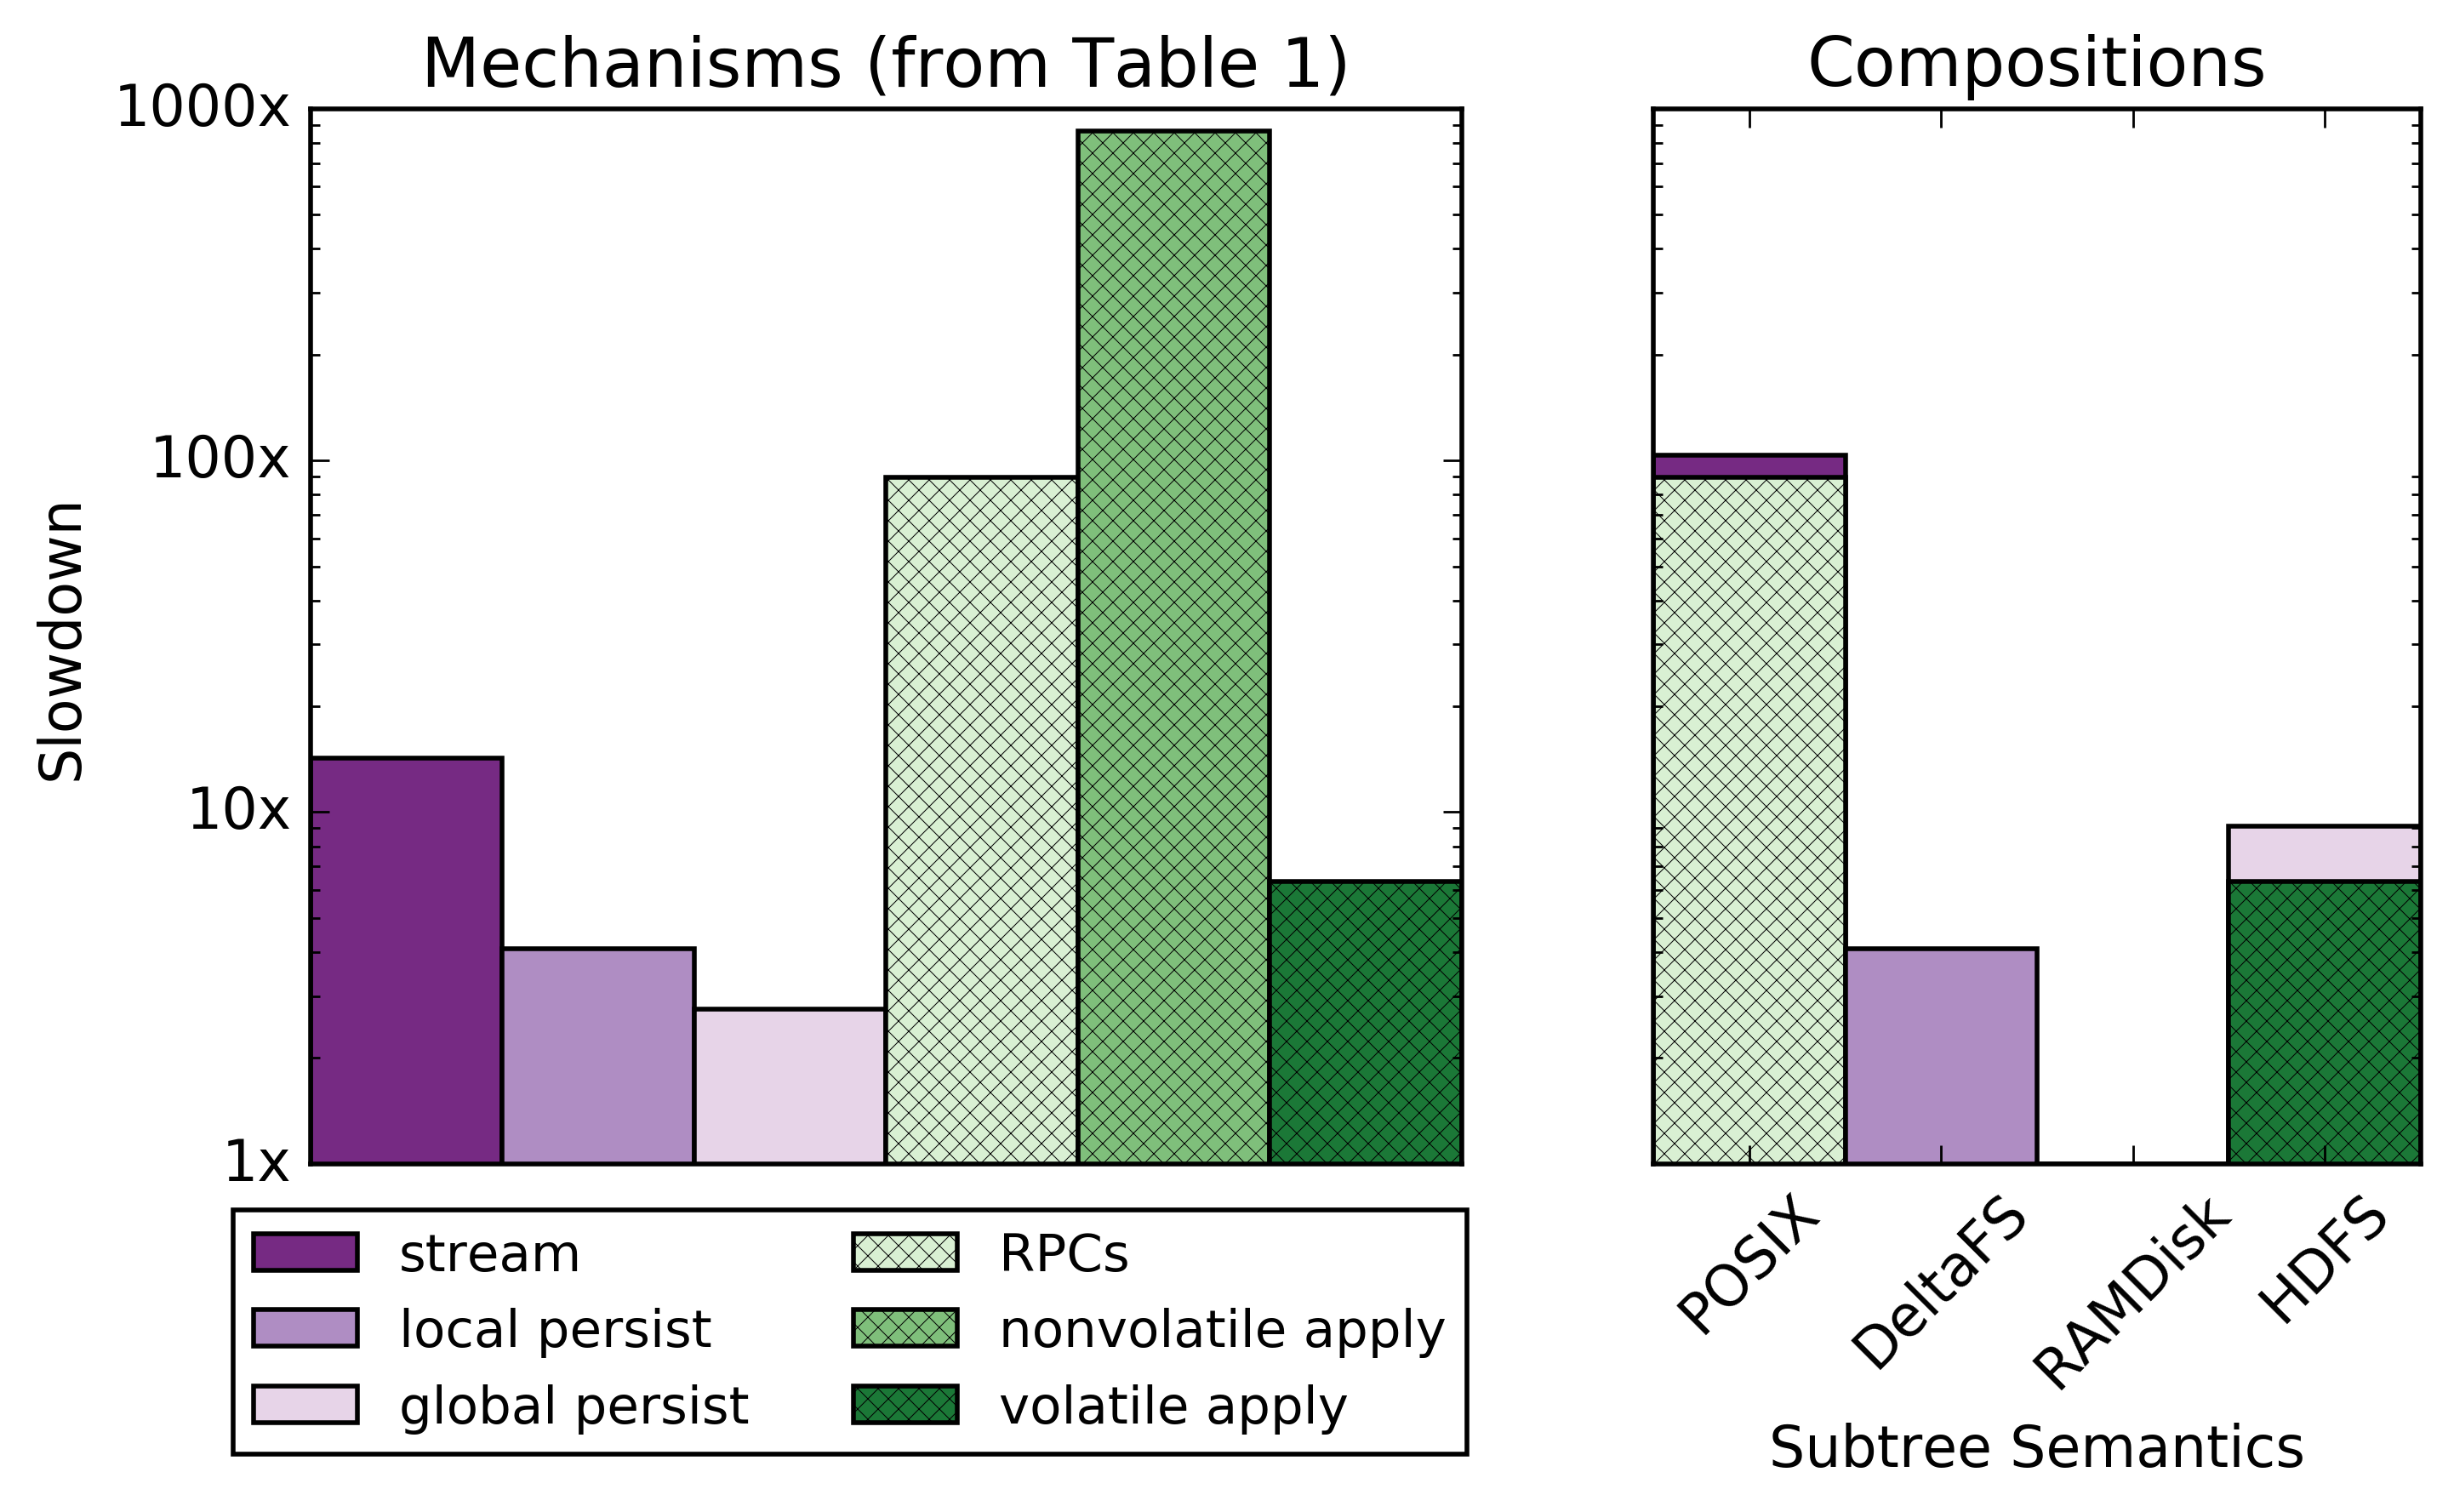
\includegraphics[width=1.0\linewidth]{graphs/composable-mechanisms.png}
\caption{ [\href{https://...}{source}] Microbenchmark: performance of each
mechanism (left) and building consistency/durability guarantees (right) for
100K files on a single client. Results are normalized to the runtime of writing
files creates to the client's in-memory journal.
\label{fig:composable-mechanisms}}
\end{figure}

\begin{figure}[tb]
\centering
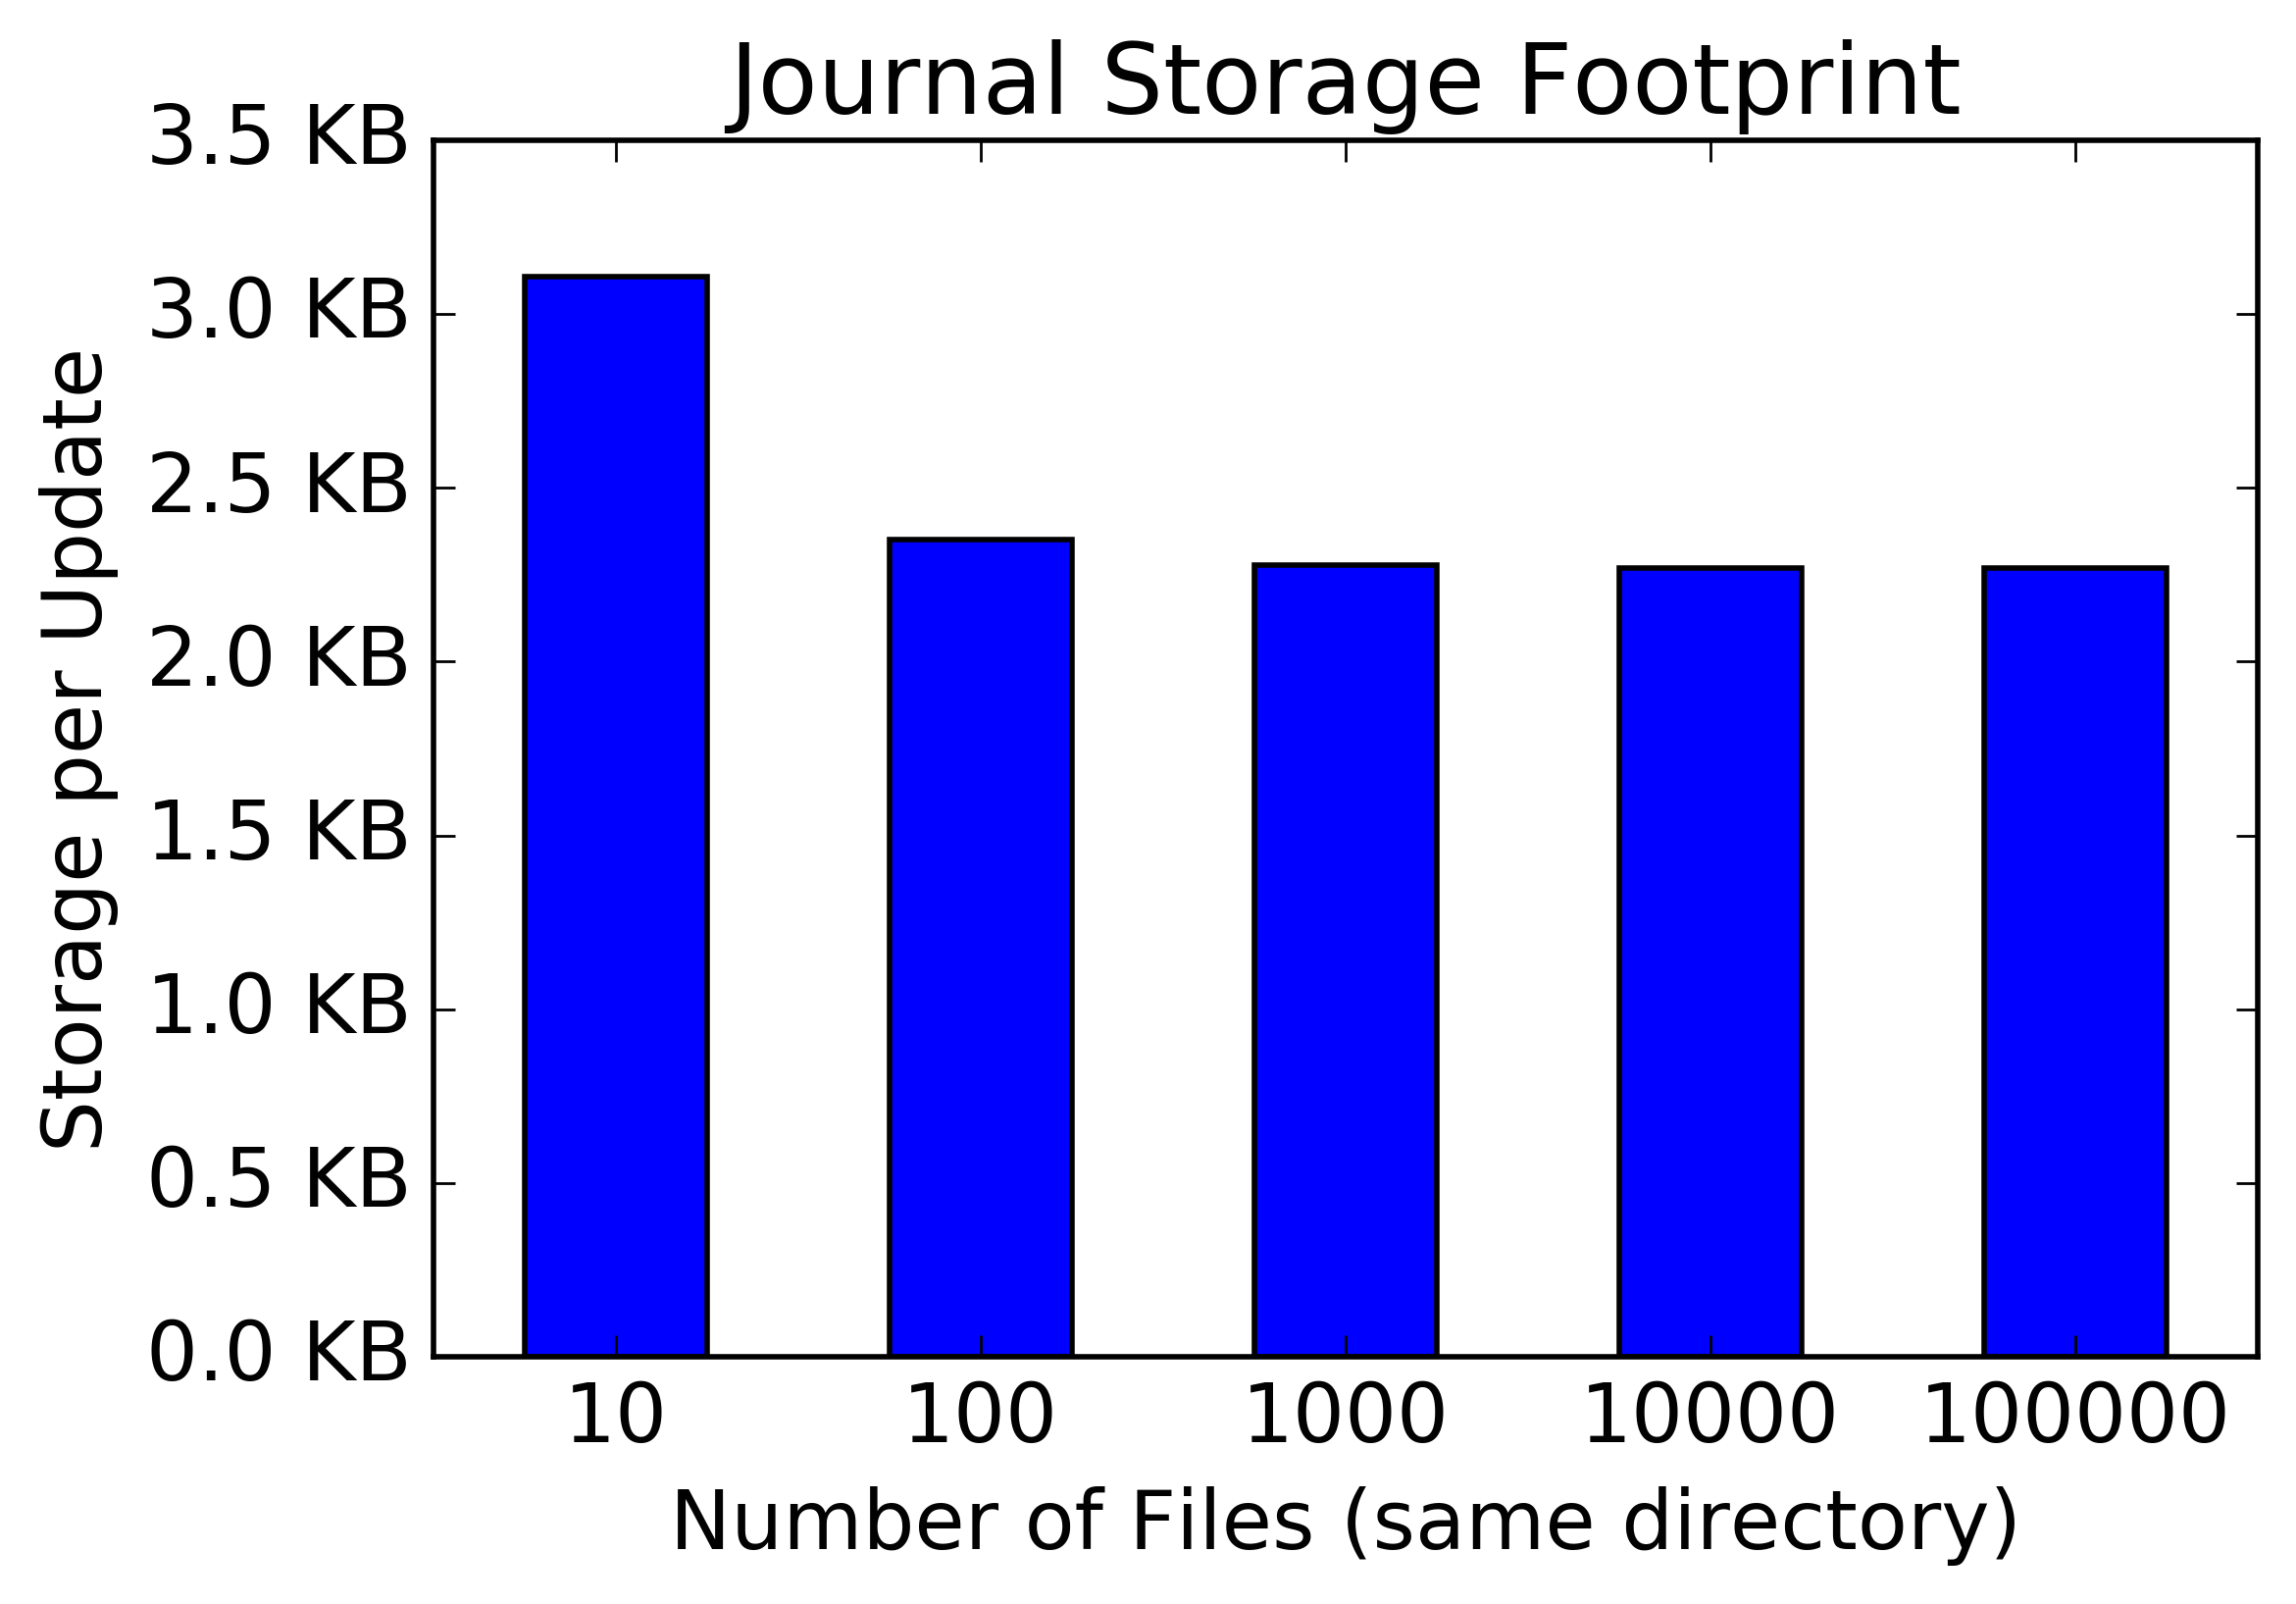
\includegraphics[width=1.0\linewidth]{graphs/behavior-journal-size.png}
\caption{ [\href{https://...}{source}] Microbenchmark: storage footprint on
client. The size of the client's journal scales with the number of
updates.\label{fig:behavior-journal-size}}
\end{figure}

Figure~\ref{fig:composable-mechanisms} shows the runtime of the Cudele
mechanisms for a single client creating files in the same directory, normalized
to the time it takes to write 100K file create updates to the client's
in-memory journal ({\it i.e.} the ``Append Client Journal" mechanism).
``Stream" is an approximation of the overhead and is calculated by subtracting
the runtime of the job with the journal turned off from the runtime with the
journal turned on.  100K is the maximum recommended size of a directory in
CephFS; preliminary experiments with larger directory sizes show memory
problems.

{\it Poorly Scaling Data Structures:} Despite doing the same amount of work,
mechanisms that rely on poorly scaling data structures have large slowdowns for
the larger number of creates. For example, ``RPCs" which relies on the internal
CephFS directory structures has a \(90\times\) slowdown for 100K files. It is a
well-known problem that directory data structures do not scale when creating
files in the same directory~\cite{ren:sc2014-indexfs} and any mechanism that
uses these data structures will experience similar slowdowns. Other mechanisms
that write events to a journal ({\it e.g.} the persists, ``Volatile Apply")
experience a much less drastic slowdown because the journal data structure does
not need to be scanned for every operation. Events are written to the end of
the journal without even checking the validity ({\it e.g.}, if the file already
exists for a create), which is another form of relaxed consistency because the
file system assumes the application has resolved conflicting updates in a
different way.

% RPCs vs. apply: calls to metadata server vs. RADOS
{\it Overhead of RPCs:} ``RPCs" is \(66\times\) slower than ``Volatile
Apply" because sending individual metadata updates over the network is costly.
While ``RPCs" sends a request for every file create, ``Nonvolatile Apply"
writes all the updates to the in-memory journal and applies them to the
in-memory data structures in the metadata server. While communicating the
decoupled namespace directly to the metadata server is faster, communicating
through the object store (``Nonvolatile Apply") is \(10\times\) slower.

% TODO: why is apply so slow.  
% apply: no CephFS changes, pulls/pushes same RADOS obj.
% v_apply vs. apply/persist: communicating through RADOS
{\it Overhead of ``Nonvolatile Apply":} The cost of ``Nonvolatile
apply" is much larger than all the other mechanisms.  That mechanism was not
implemented as part of Cudele -- it was a debugging and recovery tool packaged
with CephFS. It works by iterating over the updates in the journal and pulling
all objects that {\it may} be affected by the update.  This means that two
objects are repeatedly pulled, updated, and pushed: the object that houses the
experiment directory and the object that contains the root directory ({\it
i.e.} \texttt{/}).  The cost of communicating through the object store is shown
by comparing the runtime of ``Volatile apply" + ``Global persist" to
``Nonvolatile Apply". These two operations end up with the same final metadata
state but using ``Nonvolatile Apply" is clearly inferior.

% persist vs. save: one disk vs. many
{\it Parallelism of the Object Store:} Comparing ``Local" and ``Global
persist" demonstrates the bandwidth advantages of storing the journal in a
distributed object store. The ``Global Persist"
performance is \(1.5\times\) faster because the object store is leveraging the
collective bandwidth of the disks in the cluster. This benefit comes from the
object store itself but should be acknowledged when making decisions for the
application; the size of the object store can help mitigate the overheads of
globally persisting metadata updates.

{\it Journal Size:} Figure~\ref{fig:behavior-journal-size} shows the
amount of storage per journal update (\(y\) axis) for the range of file creates
we tested (\(x\) axis). The increase in file size is linear with the number of
metadata creates and suggests that updates for a million files would be
\(2.5\text{KB}*1\text{ million files} = 2.38\text{GB}\). Transfer times for
payloads of this size on an HPC network are reasonable.\\

\noindent\textbf{Takeaway}: measuring the mechanisms individually shows that
their overheads and costs can differ {\it by orders of magnitude}. Cudele gives
users the ability to quantify the performance impact of different
consistency/durability guarantees.\\

\subsection{Use Case 1: Creates in the Same Directory}
\label{sec:use-case-1}

% CITEME xiao:socc2015-shardfs CITEME HADOOP
Clients creating files in private directories is heavily studied in
HPC~\cite{weil:sc2004-dyn-metadata, ren:sc2014-indexfs, patil:fast2011-giga,
zheng:pdsw2014-batchfs, sevilla:sc15-mantle}, mostly due to
checkpoint-restart~\cite{bent_plfs_2009}.  But the workload also appears in
cloud workloads, where systems like Hadoop use the file abstraction to exchange
work units to workers or to indicate when jobs
complete~\cite{shvachko:login2012-hdfs-scalability}. A more familiar example is
uncompressing an archive ({\it e.g.}, \texttt{tar xzf}), where the file system
services a flash crowd of creates across all directories as shown in
Figure~\ref{fig:overhead-creates}.  We use this as a microbenchmark because it
allows us to control the size of the log, since each create creates a single
journal event.

%\begin{figure}[tb]
%\centering
%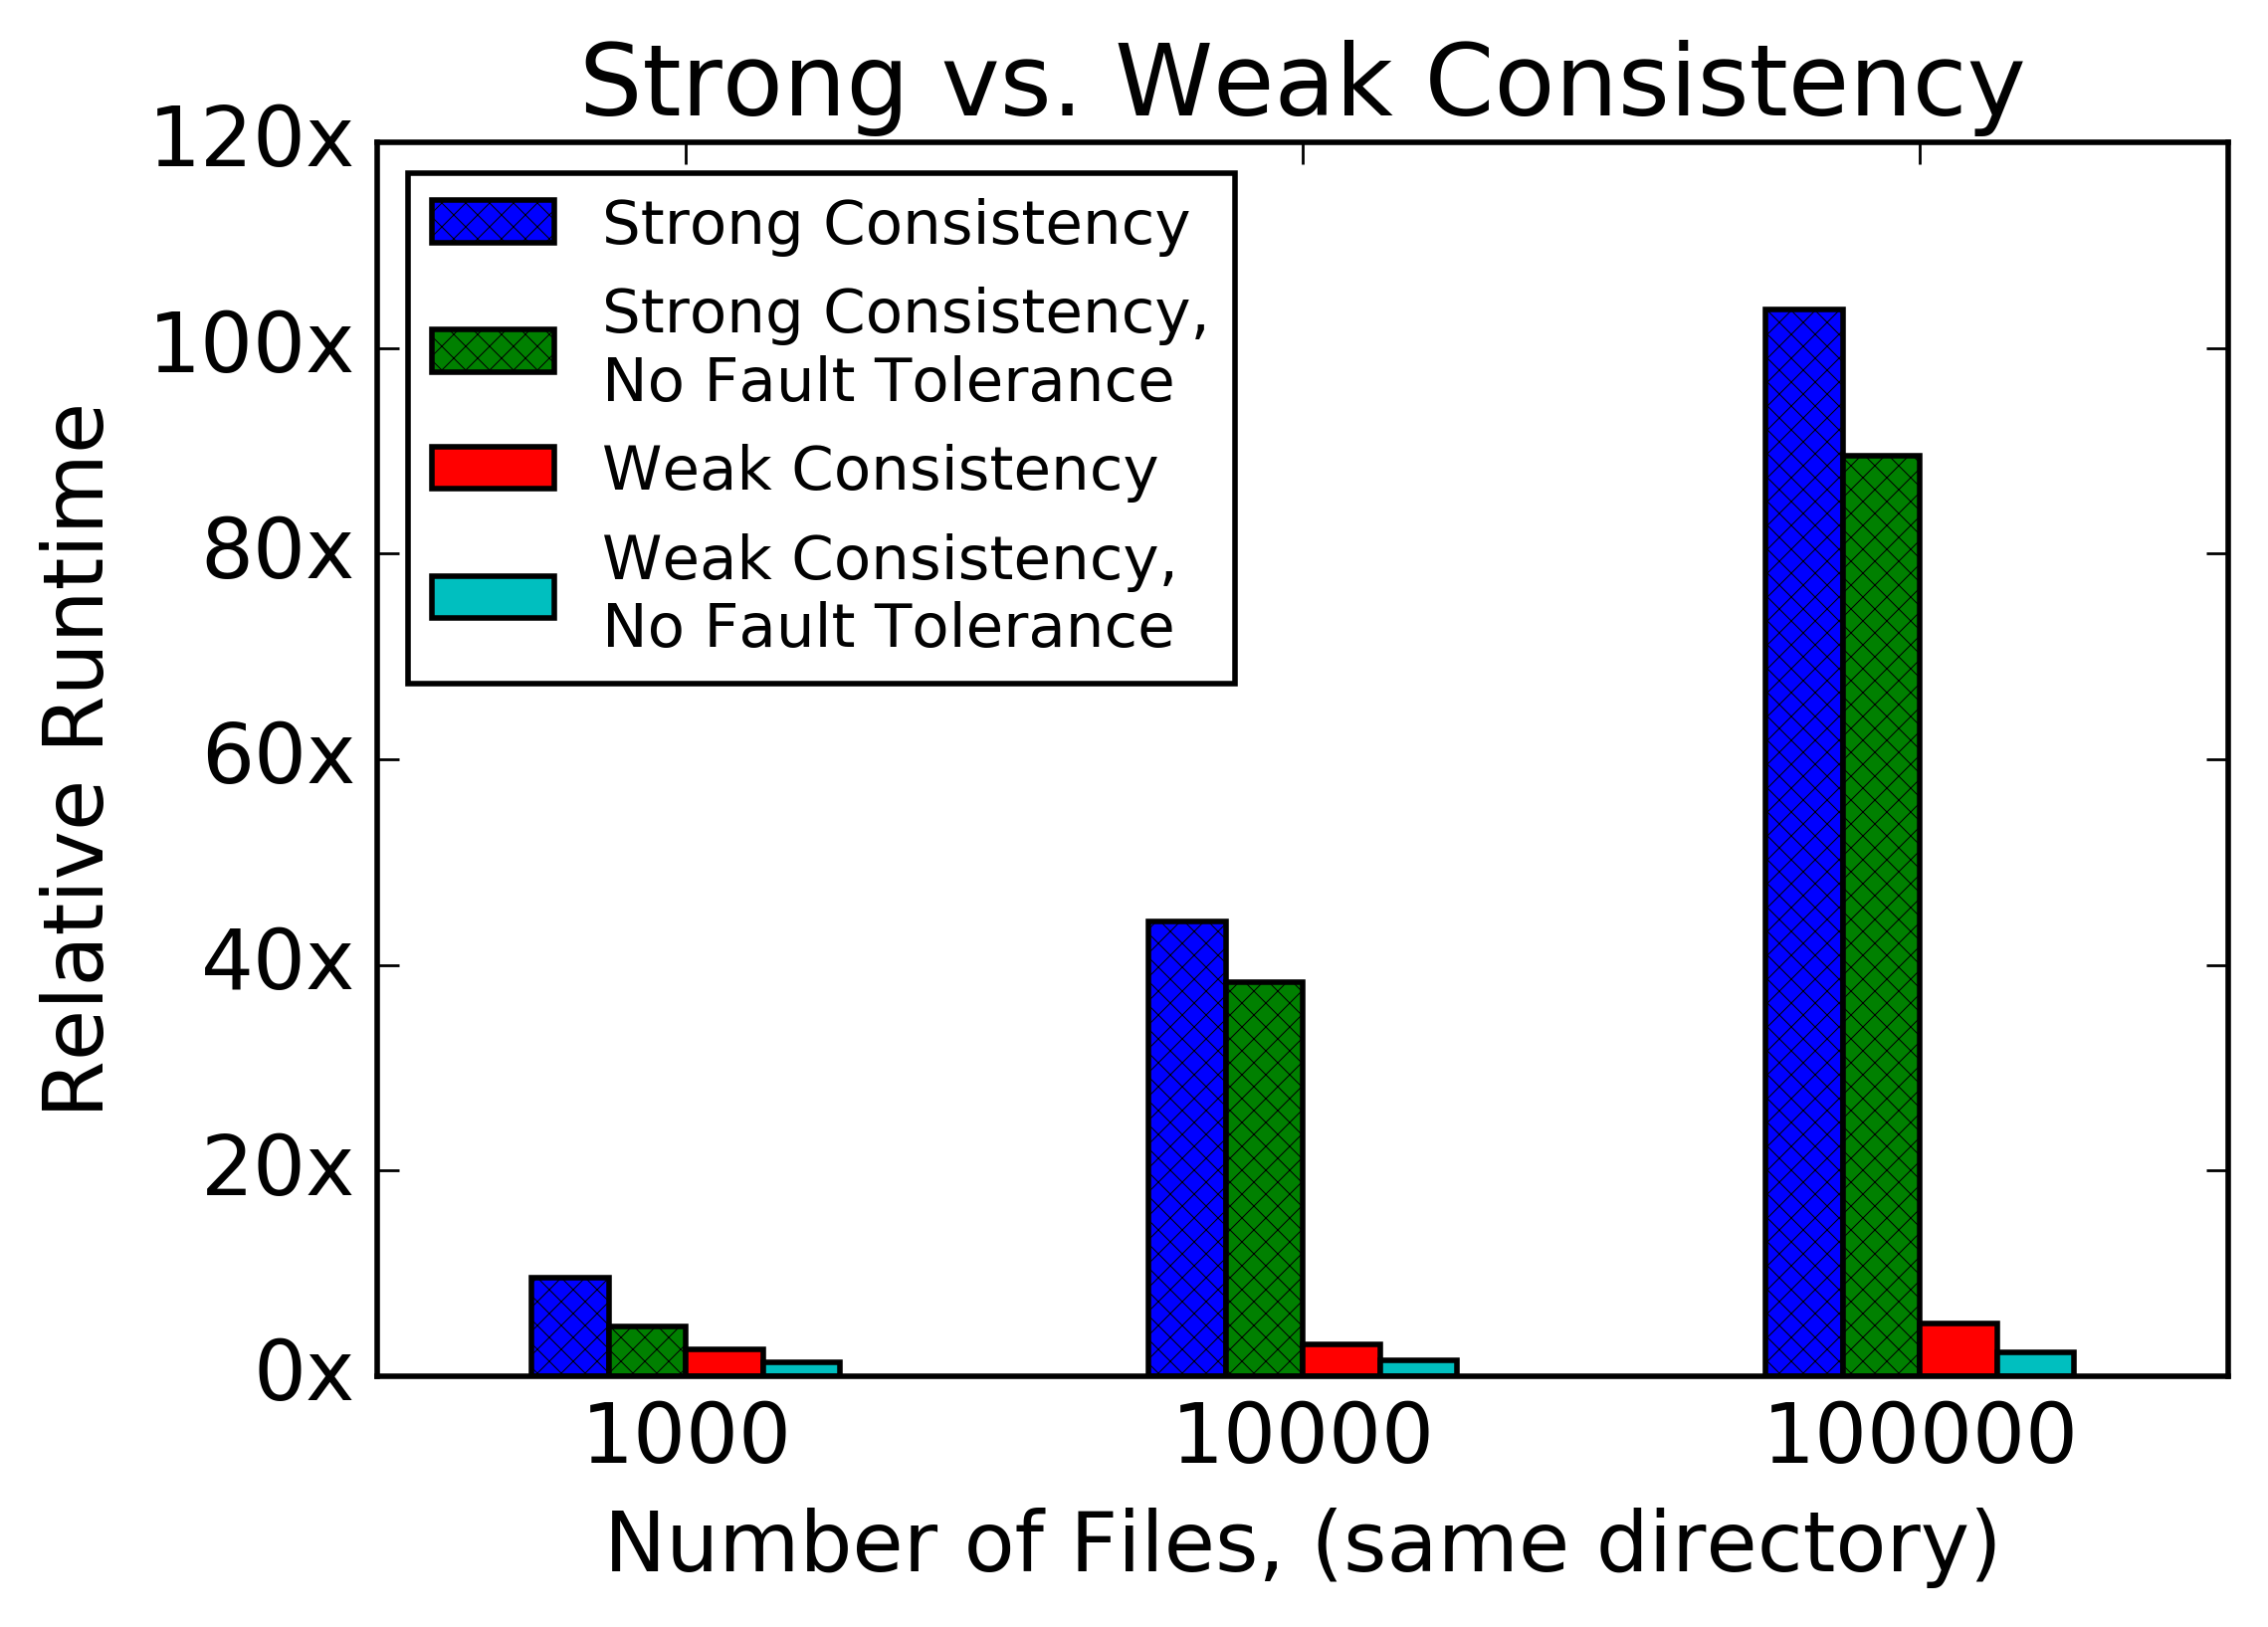
\includegraphics[width=1.0\linewidth]{graphs/slowdown-strong-v-weak.png}
%\caption{ [\href{https://...}{source}] Use Case 1: the RPC per metadata update
%(strong consistency) has a large overhead compared to decoupled namespaces
%(weak consistency.)\label{fig:slowdown-strong-weak}}
%\end{figure}

The graph on the right of Figure~\ref{fig:composable-mechanisms} shows how
applications can compose mechanisms together to get the consistency/durability
guarantees they need.  We label the \(x\)-axis with systems that employ these
semantics, as described in Figure~\ref{fig:subtree-policies}.  Again, the
runtime of different semantics for subtrees in the same global namespace
normalized to the runtime of the ``Append Client Journal" mechanism (again,
just creating files in the client's in-memory journal).  We makes no guarantees
during execution of the mechanisms or when transitioning semantics -- the
semantics are guaranteed {\it once the mechanism completes}. So if servers fail
during a mechanism, metadata or data may be lost.

%% DeltaFS vs. BatchFS vs. POSIX: decoupled is faster
%% (5-7x) vs. (90-104x) slower
%% Does not scale?
%% Strong Consistency > 10X slower than Weak Consistency 
%{\it Speedups of Decoupled Namespaces:} Weak consistency uses the
%decoupled namespace strategy and shows up to a \(20\times\) speedup over the
%traditional namespaces that use RPCs. Compared to the baseline the slowdown is
%\(5-7\times\) for Strong Consistency, which emulates BatchFS and
%\(90-104\times\) for Weak Consistency, which emulates DeltaFS.

{\it Durability \(<<\) Consistency:} The performance of these semantics
suggests that the overhead of consistency is much larger than the overhead of
durability. This conclusion should be stronger as we scale the number of files
because the cost of streaming the journal into the object store is constant.

% Weak Consistency benefit not due to metadata format
{\it Metadata Formats:} Because the metadata formats are the same for
all schemes we argue that the performance gain for decoupled namespaces comes
from relaxing the consistency guarantees and not from the metadata formats.\\

\noindent\textbf{Takeaway}: we confirm the performance benefits of other
well-established research systems but, more importantly, we show that the
Cudele mechanisms we propose are useful for building evaluating different
consistency/durability semantics.

%\section{notes}
%Linking clients into our custom libcephfs
%
%Use namespace's recursive data structure to put policies on subtrees
%- consistency: weak vs. strong, global vs. local
%  - e.g., BatchFS/DeltaFS: weak, local
%  - e.g., POSIX: strong, global
%  - e.g., PLFS: no consistency
%- durability: global vs. local
%  - e.g., CephFS: global
%  - e.g., BatchFS/DeltaFS: local
%
%Experimental Setup
%- Ceph: 9 OSDs, 1 metadata server, 2 kernel client
%- Workload limitations: blah
%
%Workload: creates
%
%Baseline: 200K creates in the same directory
%- throughput: degrades at 950s
%- CPU utilization: more at 950s
%- inode cache: eviction dominate
%- inodes +- to cache: eviction dominate
%- per-disk throughput: RADOS not bottleneck
%
%Experiment 1: Interference
%
%\subsection{Baseline}
%Experiment 0: creates in the same directory
%- setup: why we use caching, we use the kernel client, how we circumvent max fragment size
%
%Experiment 0: creates with a stat
%- Hypothesis: metadata read pauses creates and requires a snapshot in time
%  - what is more of an overhead: pausing creates and getting a consistent view OR sucking up resources as it reads from RADOS?
%- can we delay snapshot?
%
%Experiment 1: creates with a readdir
%- Hypothesis: shows the cost of synchronization because on a write, the first client drops his caps
%- client0: create 100k, client1: stat at 2 mins
%
%Experiment 2: scale the number of files
%- See if the open/close spike occurs 
%- Try to see why open/close spike is allowed to happen
%- Try to disable all caching -- metadata writes don't ever re-use the inode -- we never ask for it again!
%- client0: create 100k, client1: touch at 2 mins
%
%Experiment 3: see how fast the cache satisfies a read
%- client0: create 100k, stat inodes
%- client0: create 100k, client1: stat inodes
%
%lient 0: creates, client 1 create(s)

\subsection{Use Case 2: Creates with Rogue Client}

Clients create files in private directories and a separate client, which we
call a ``rogue" client, creates files in each directory. This introduces false
sharing and the metadata server revokes capabilities on directories touched by
the rogue client. While HPC tries to avoid these situations with
worklflows~\cite{zheng:pdsw2014-batchfs, zheng:pdsw2015-deltafs}, it stills
happens in distributed file systems when users unintentionally access
directories in a shared file system.

\begin{figure}[tb]
\centering
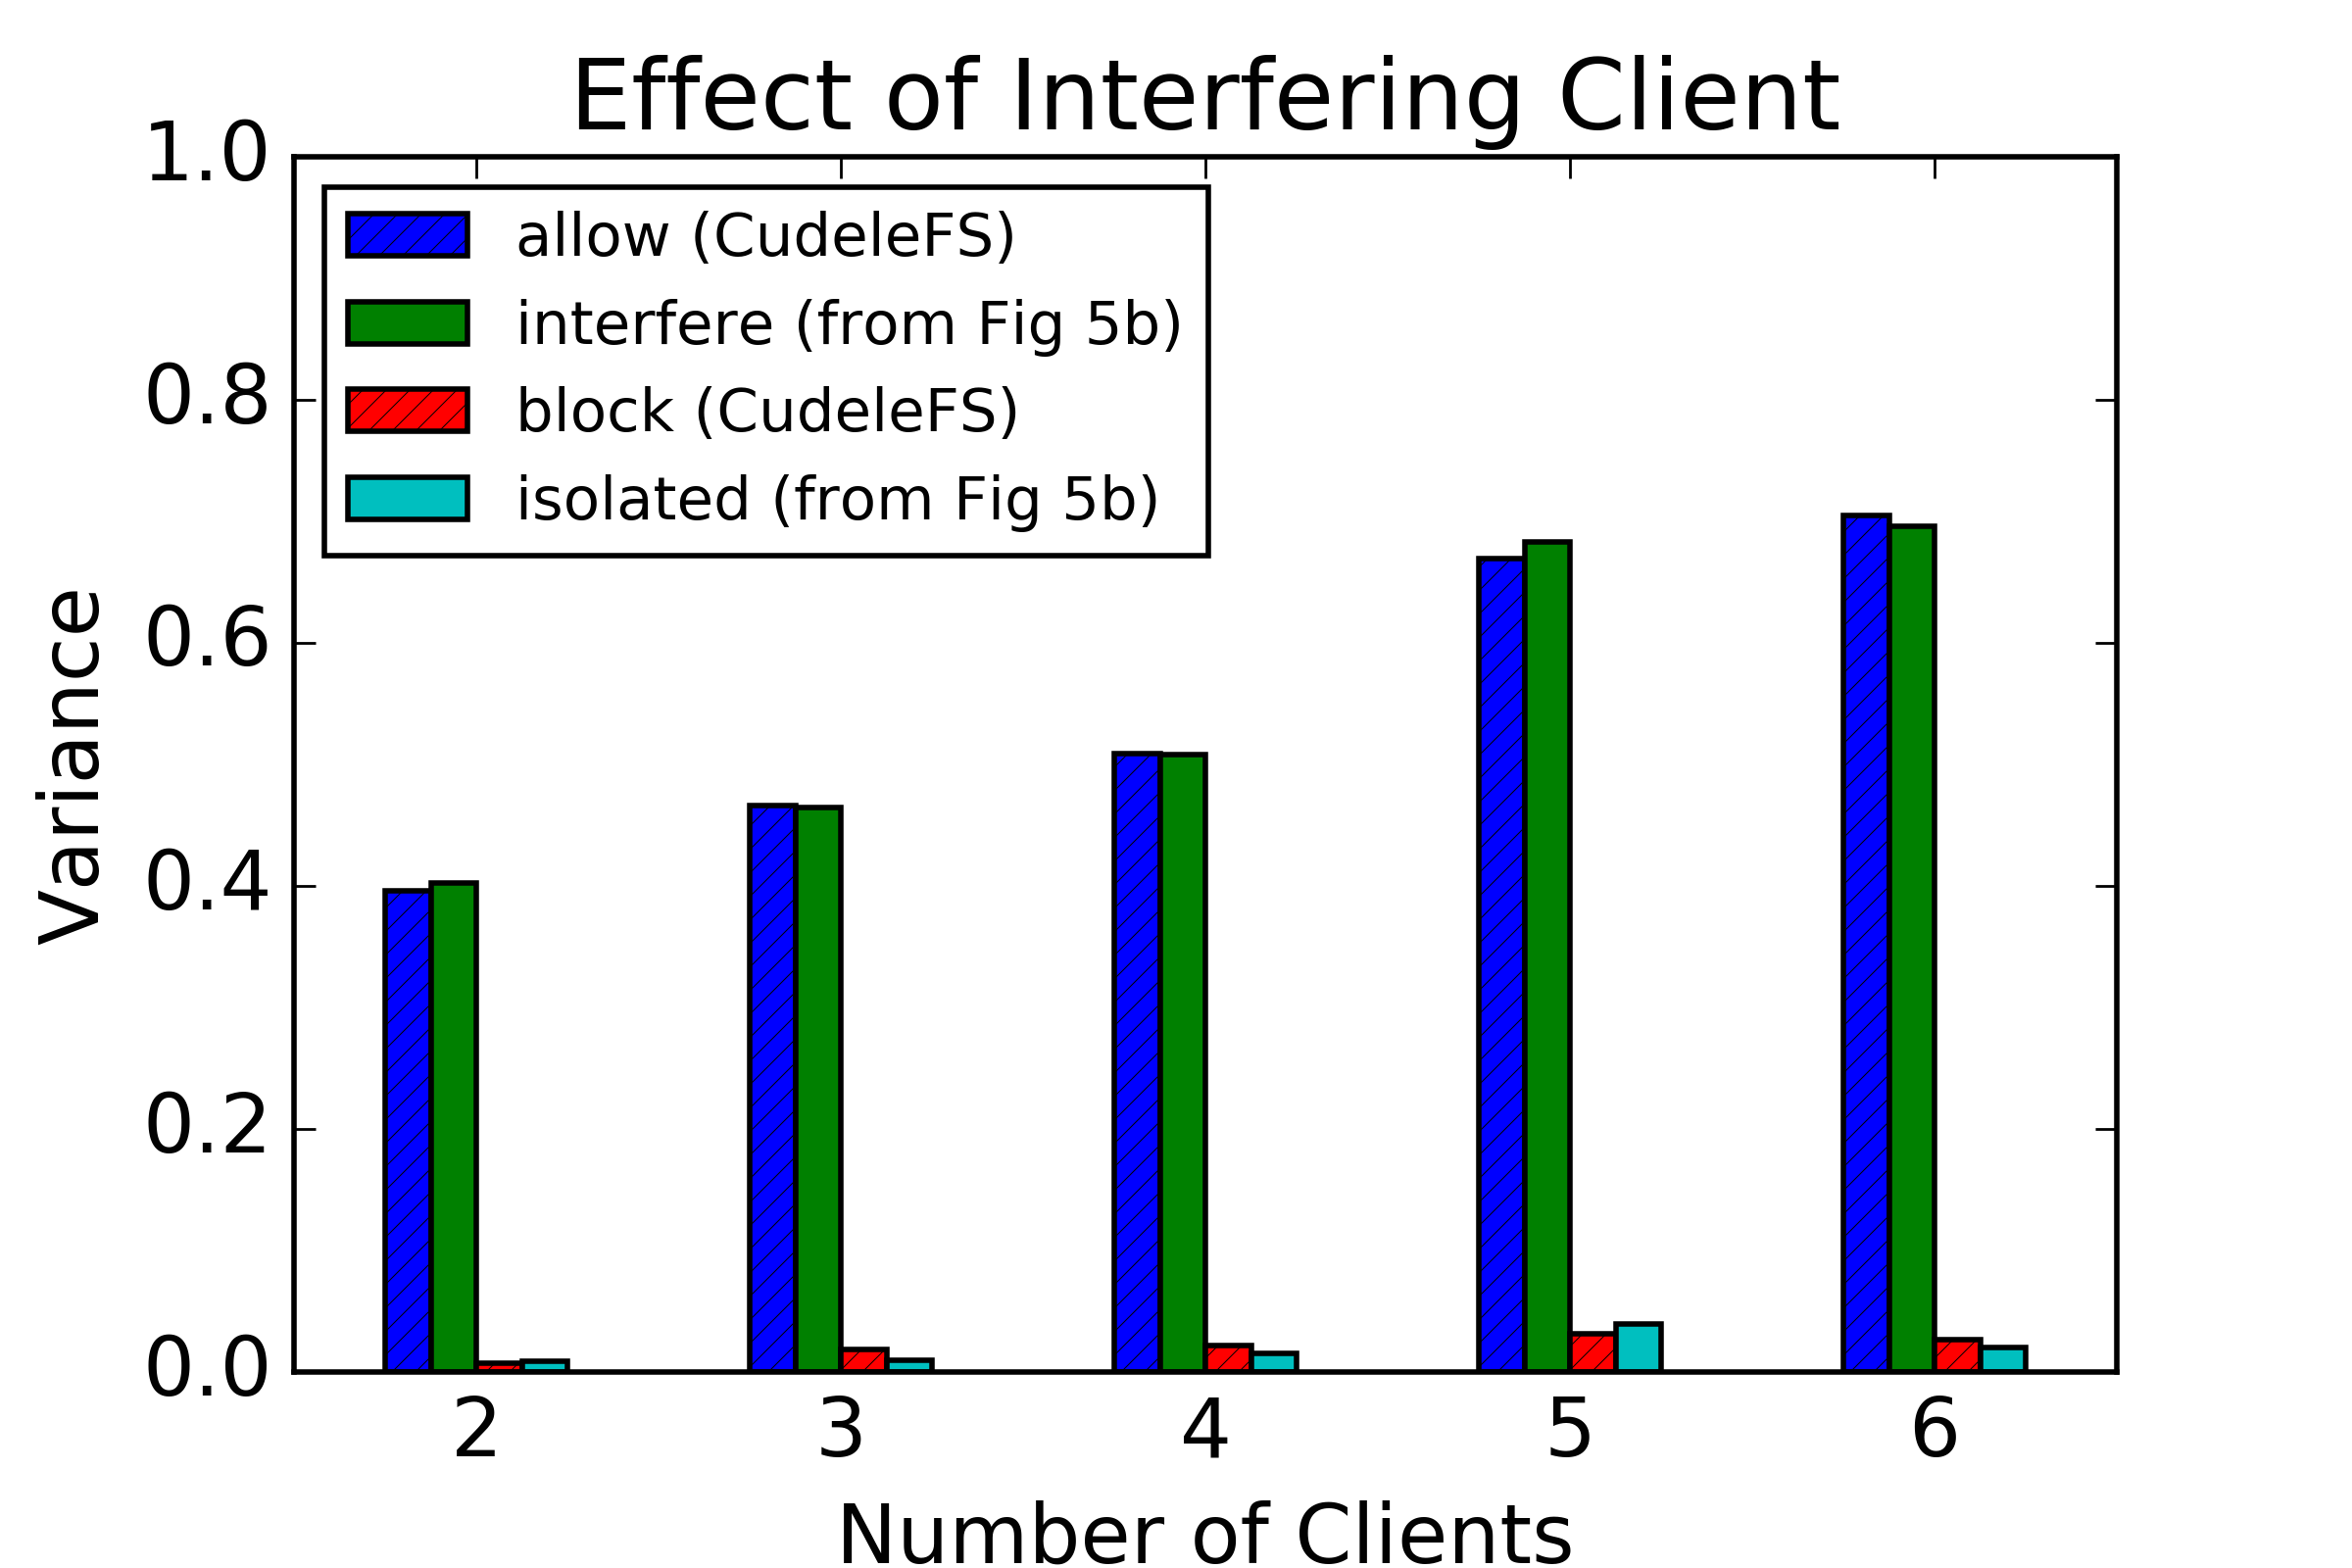
\includegraphics[width=1.0\linewidth]{graphs/slowdown-allow-block.png}
\caption{ [\href{https://...}{source}] Use Case 2: using the ``allow" and
``block" API, users can isolate directories from interfering clients. Variance
with blocking turned on is the same as ``isolated" from
Figure~\ref{fig:overhead-b}.
\label{fig:slowdown-allow-block}}

\end{figure}

% setup: 2cs sep dirs, 2cs DN, 1c malicious write
Next we show how Cudele can be programmed to block interfering clients. We
use the same problematic workload from Figure~\ref{fig:overhead-b}, where
clients write to their own private directories and another client interferes with a stream of creates at
30 seconds.  We also have another client write to a decoupled namespace and
merge its updates at 90 seconds.  We equip each client directory with the
configuration:

\begin{listing}[tb]
\begin{minted}[xleftmargin=21pt,
               tabsize=4]{js}
{     
    "allocated_inodes": "100000"
    "interfere_policy": "block"
    "consistency": "RPCs"
    "durability": "stream"
}
\end{minted}
\end{listing}

Each directory functions with ``RPCs"
and ``Stream" enabled -- which is the default implementation of CephFS. The only
difference is that we enable blocking on each subtree so while the tree behaves
like CephFS, all interfering operations will be returned with \texttt{-EBUSY}.
Note that IndexFS does a similar operation with leases except clients block.

% results
To show the benefits of this isolations, our results in
Figure~\ref{fig:slowdown-allow-block} are plotted alongside the variance bars from
Figure~\ref{fig:overhead-b}. Because ``allow"/``interfere and
``block"/``isolated" have the same variability we draw the following three
conclusions: (1) clients that use the API to block interfering clients  get
the same performance as isolated clients, (2) there is a negligible effect on
performance for the extra work the metadata server does to return
\texttt{-EBUSY}, and (3) merging updates from the decoupled client has a
negligible effect on performance.\\

\noindent\textbf{Takeaway}: the API lets users isolate directories when
applications need better and more reliable performance. This is a way of
controlling consistency.

\subsection{Use Case 3: Read while Writing}

% CITEME
Scientists use the file system to check the progress of jobs using
\texttt{ls}~\cite{CITEME}. The number of files or size of the files is
indicative of the progress. This practice is not too different from systems
that use the file system to manage the progress of jobs; Hadoop writes to
temporary files, renames them when complete, and creates a ``DONE" file to
indicate to the runtime that the task did not fail and should not be
re-scheduled on another node. In this scenario, Cudele users will not see the
progress of decoupled namespace since their updates are not globally visible.
To help scientists judge the progress of their jobs, Cudele clients have a
``namespace sync" that sends batches of updates back to the global namespace at
regular intervals.

\begin{figure}[tb] \centering
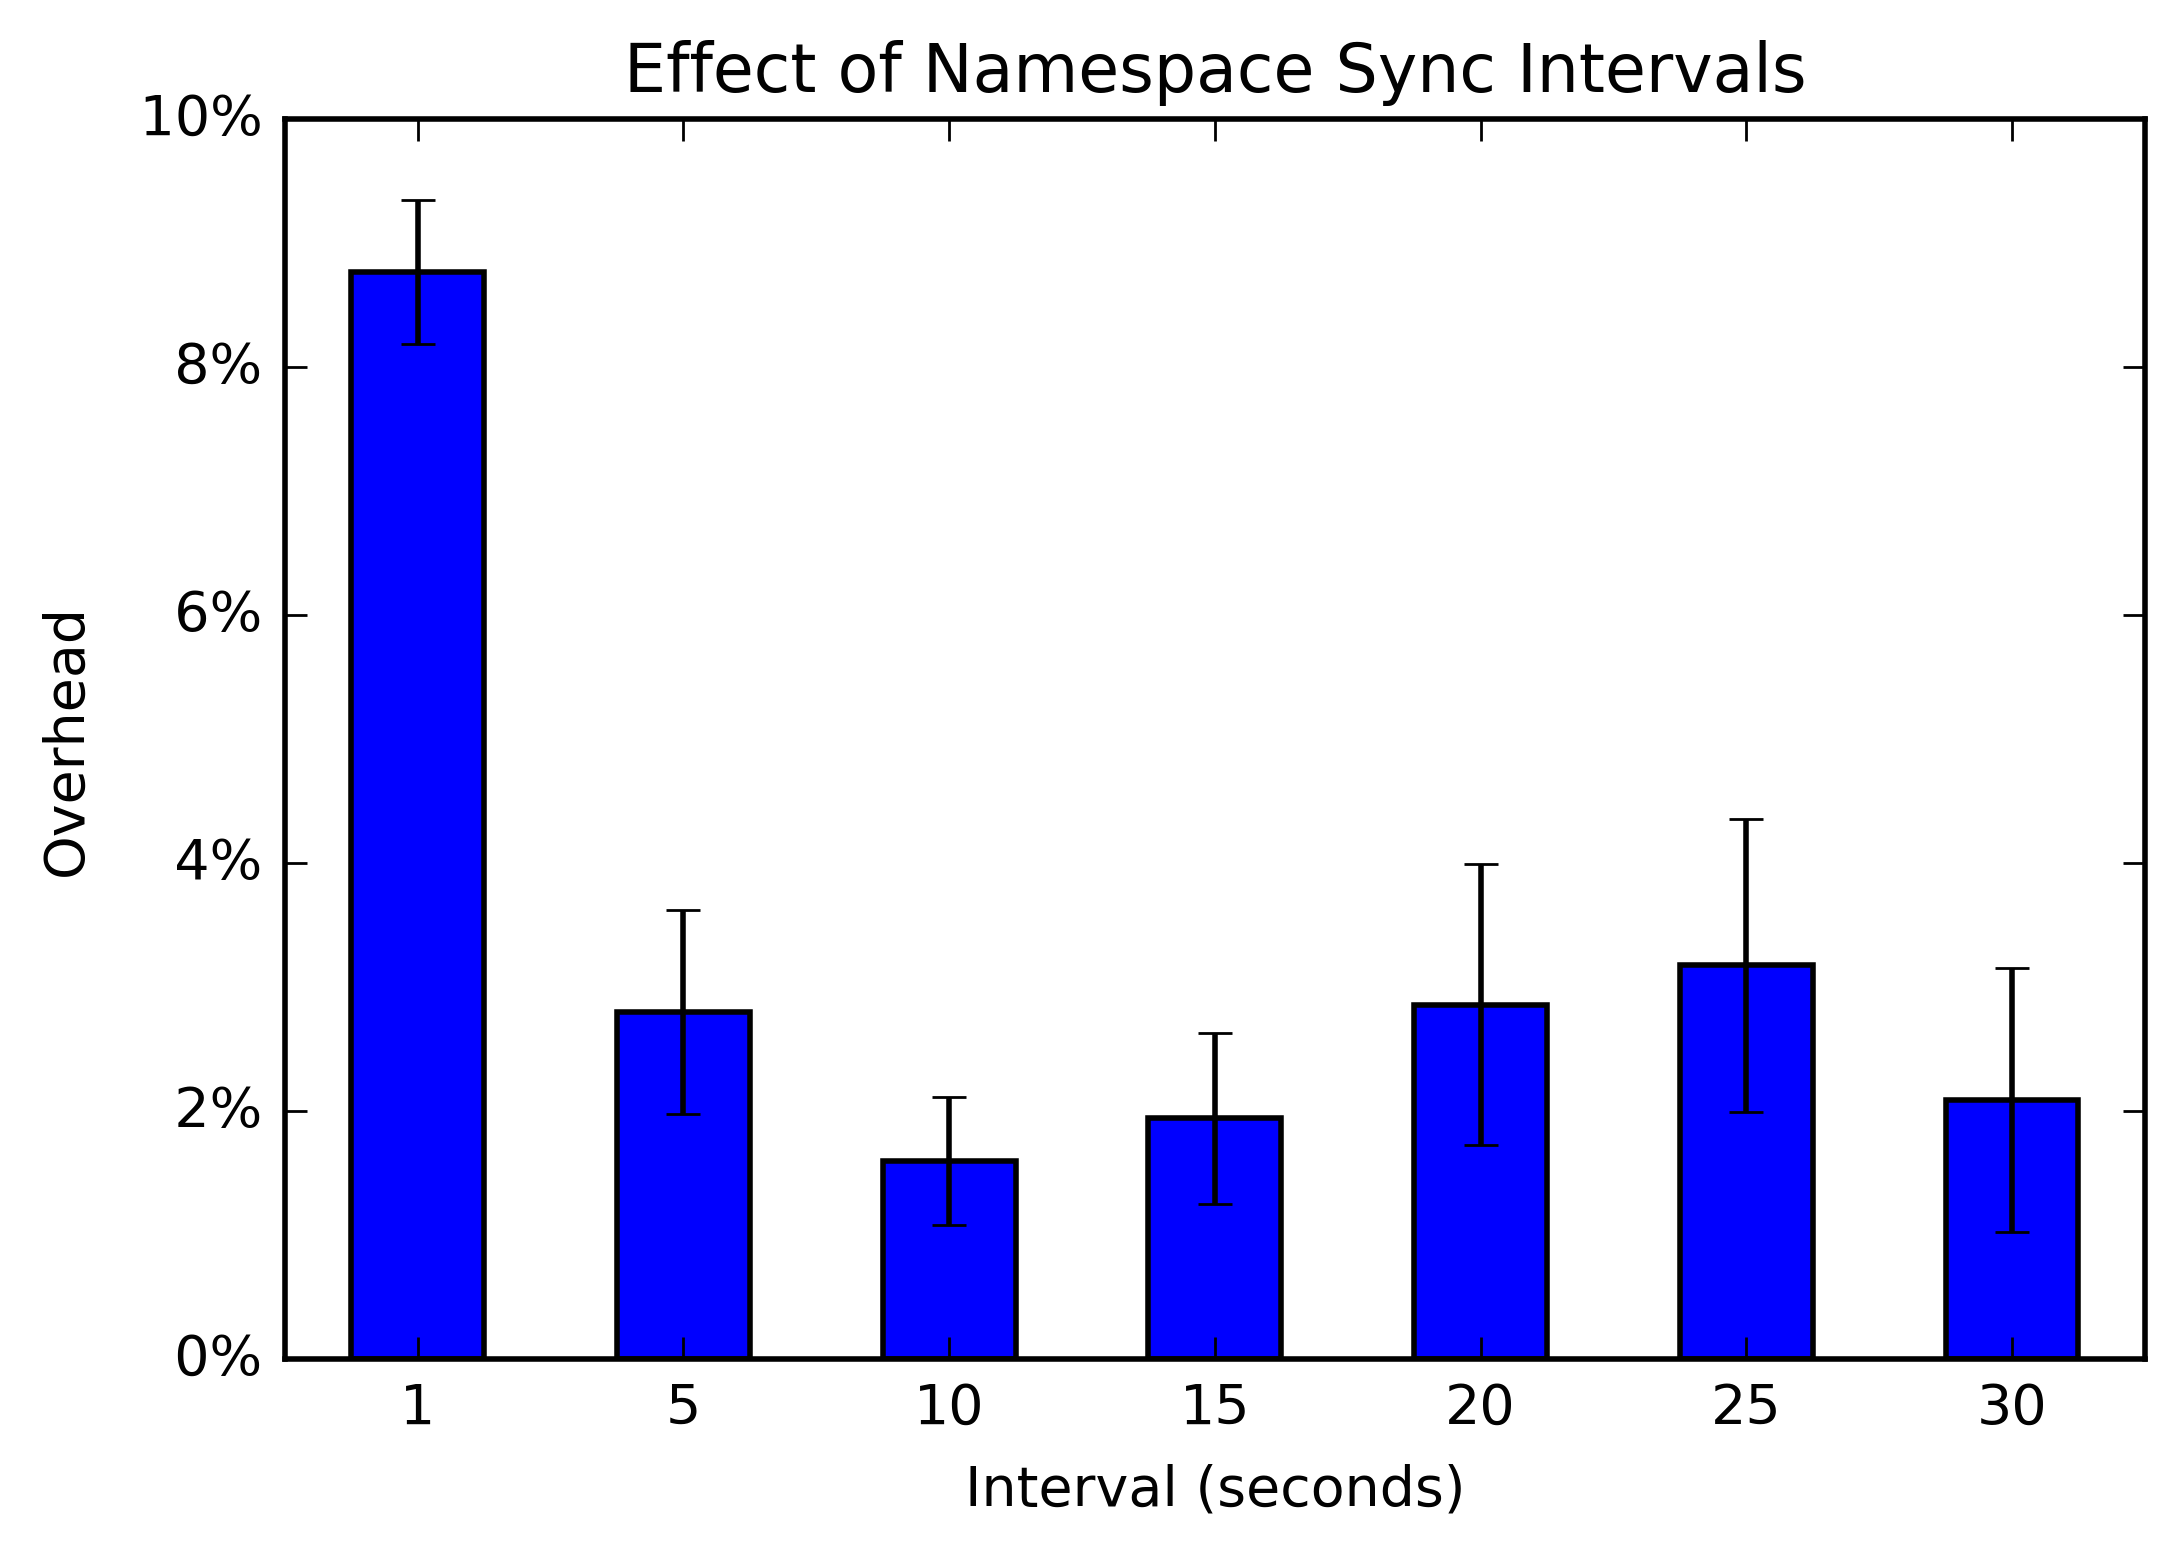
\includegraphics[width=1.0\linewidth]{graphs/slowdown-sync.png} \caption{
[\href{https://...}{source}] Use Case 3: slowdown of a single client periodically syncing
updates to the gobal namespace. The crossover point represents the trade-off of
frequent updates (with small journal files) and infrequent updates (with larger journal
files).\ref{fig:slowdown-sync}.  \label{fig:slowdown-sync}}
\end{figure}

\begin{figure}[tb] \centering
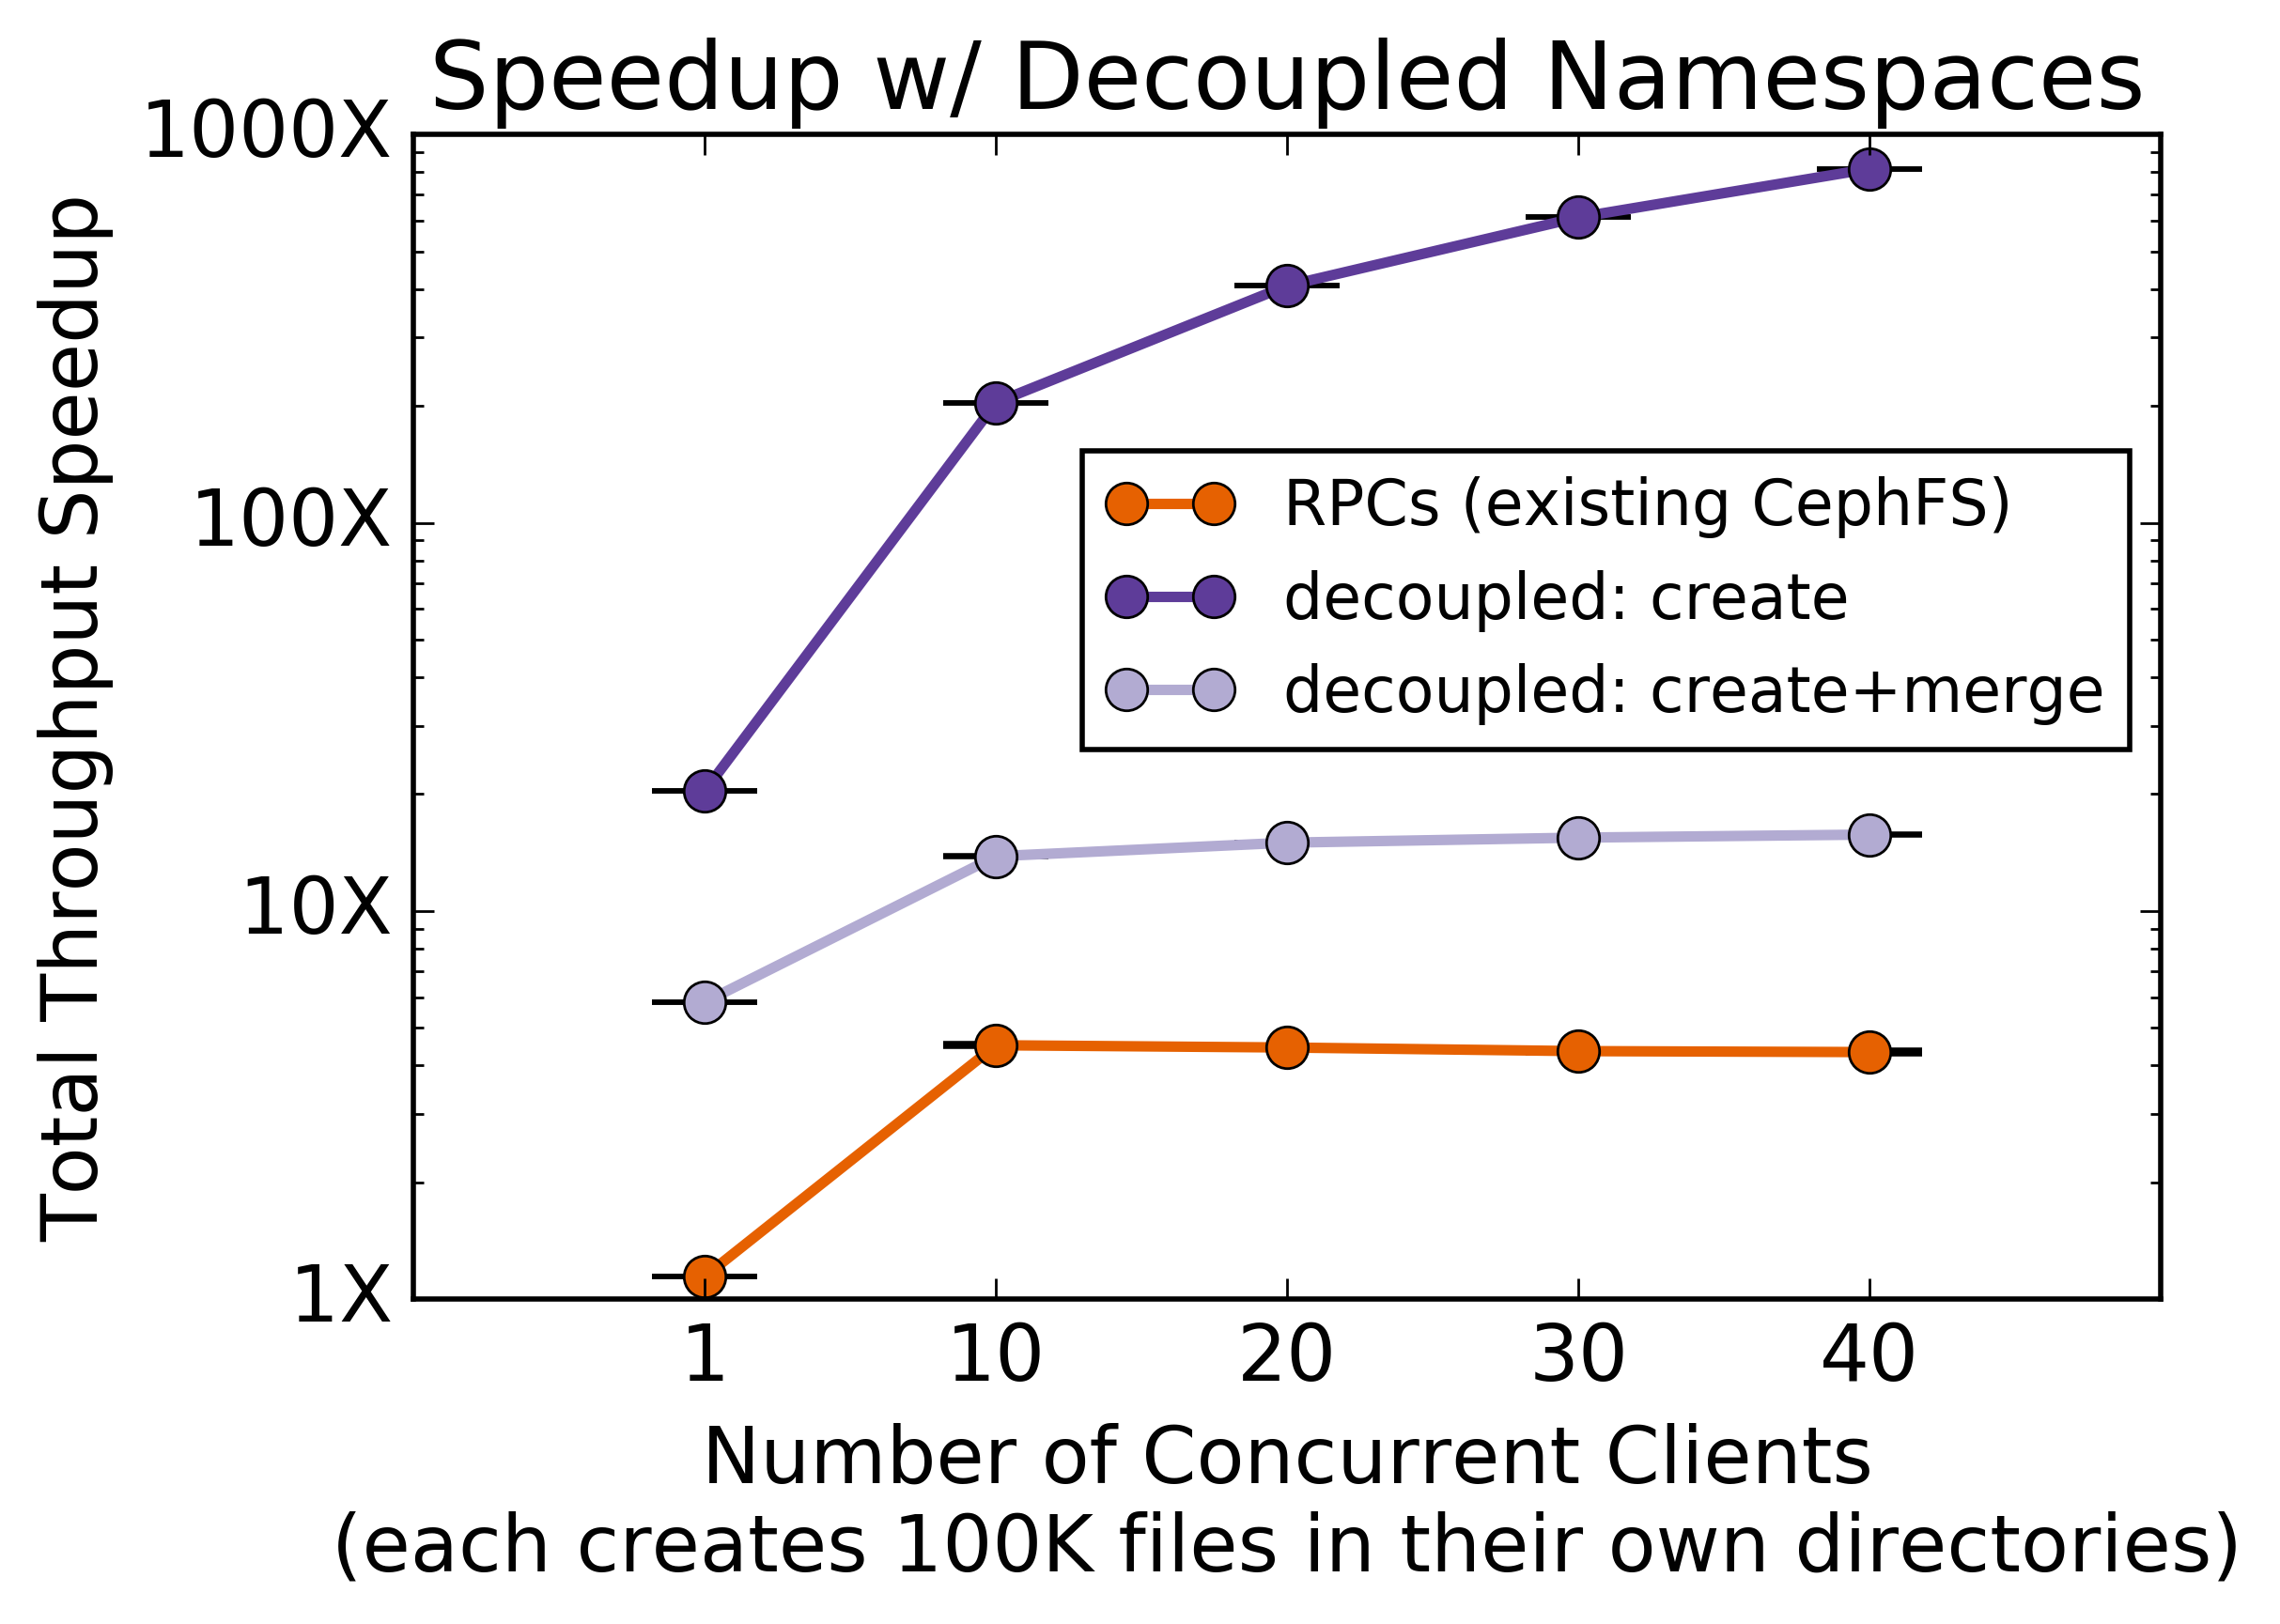
\includegraphics[width=1.0\linewidth]{graphs/mergescale.png} \caption{
[\href{https://...}{source}] Use Case 3: performance of merging client journals
at the metadata server. Performance is better than RPCs because (1) there are
less messages on the network and (2) the consistency/durability code paths in
the metadata server are bypassed. Merges are serialized and read from the local
disk, so keeping client journals in memory or on SSD will improve the
performance of ``decoupled" even more.  \ref{fig:mergescale}.
\label{fig:mergescale-sync}}
\end{figure}

% Does this implementation need to be described in the implementation?
Figure~\ref{fig:slowdown-sync} shows the performance degradation of a single
client writing updates to a decoupled namespace and pausing to send updates to
the metadata server. We scale the namespace sync interval to show the trade-off
of frequently pausing or writing large logs of updates.  We use an idle core to
log the updates and to do the network transfer. The client only pauses to fork
off a background process, which is expensive as the address space needs to
copied. The alternative is to pause the client completely and write the update
to disk but since this implementation is limited by the speed of the disk, we
choose the memory-to-memory copy of the fork approach.

To show the contention at the metadata server of this approach, we scale the
number of journal merge events, each hitting different directories in the
namespace, in Figure~\ref{fig:mergescale}. The size of each journal is 100K
files, the maximum recommended directory size for CephFS. We also plot the cost
of RPCs with and without journaling; recall from Figure~\ref{fig:overhead-c}
that the scalability that max number of clients that the default metadata
server could support with RPCs is 18.

Merge requests are serialized at the metadata server; merging concurrently is
an optimization for future work. The current implementation has race conditions
because the metadata server recovery code was not designed to run in parallel
({\it i.e.} the metadata server never recovers with multiple threads). As a
result, the metadata server versions inodes and directory entries to ensure
that the recovered metadata is consistent.

Performance is better than RPCs because we place no restrictions on the
validity of metadata inserted into the journal and avoid touching poorly
scaling data structures. In other words, we can scale linearly if we weaken our
consistency by never checking for the existence of files before creating files.
only appends \texttt{open()} requests to the journal. When the updates are
merged by the metadata server into the in-memory metadata store they never scan
growing data structures.  Had we implemented the ``Create" mechanism to include
\texttt{lookup()} commands before \texttt{open()} requests, we would have seen
the poor scaling that we see with the ``RPCs" mechanism.\\

\noindent\textbf{Takeaway}: the weakest form of consistency for creating files
({\it i.e.} not checking data structures for the validity of an update or
existence of a file) shows linear scalability and stable performance.

\subsection{Use Case 4: Reading Large Directories} 

% CITEME
The final use case is reading large directories. At job completion, scientists
might use \texttt{ls} again to see the results. This causes great strain on the
file system as paths need to traversed and the entire directory, with all its
entries, must be transferred back to the client. Here we show how decoupling a
large namespace and materializing the view in memory on the client is faster
than doing RPCs for walks of the file system namespace.

FigureX shows how fast a client can materialize decoupled namespaces in memory.
This takes the on-disk file system metadata format and parses them into events
that can be manipulated and appended to. Again, we scale the number of up

\subsection{Discussion}
\begin{itemize}
  \item Composable guarantees: applications control their performance (knobs you didn't have before)
  \item Hardware features: adding hardware in strategic places
  \item Performance Prediction: quantifies the cost of each mechanism
\end{itemize}
